\chapterimage{chapter_head_1.png}

\chapter{Sprachverarbeitung}
\section{Einleitung}
Sprache ist ein natürliches Kommunikationsmittel, das der Übermittlung von Informationen dient.
Es liegt daher auf der Hand, Sprache auch zur Kommunikation mit Computern nutzen zu wollen.
Zeichenketten sind als Eingaben gang und gäbe.
Interessant für den Bereich der künstlichen Intelligenz werden solche Eingaben, wenn sie eine Interaktion mit einem Rechner ermöglichen, die nicht nur streng formal definierte und eng begrenzte Eingaben, sondern eine möglichst große Teilmenge einer natürlichen Sprache erlaubt.
Dies setzt voraus, dass der Rechner in der Lage ist, die Eingabe zu analysieren und zu interpretieren.
Insbesondere ist auch die gesprochene Kommunikation mit Computern ein aktueller Trend.
Diese Eingabeschnittstelle gewinnt insbesondere durch die zunehmende Nutzung mobiler, tastaturloser Geräte in Form von Sprachassistenten wie Siri, Cortana und Google Now an immenser Bedeutung.
Aber auch die Sprachsteuerung von Unterhaltungselektronik und Haushaltsgeräten (smart homes) sowie von Automobilen, die verstärkt computerisiert ausgestattet sind und sich während der Fahrt am besten per Sprache bedienen ließen\footnote{Zumindest solange wir noch nicht von selbstfahrenden Autos reden.}, sind hier zu nennen.
Hier befassen wir uns mit zwei Formen von Sprache: gesprochene Sprache und Texte.\footnote{Darüber hinaus gibt es natürlich noch weitere Möglichkeiten sprachlicher Kommunikation, etwa Körpersprache und Gebärdensprache, für die aber wiederum andere Methoden der digitalen Erfassung notwendig wären.}

Texte sind Folgen von Buchstaben und Zeichen aus einem gegebenen Alphabet.
Die Menge der in einer Sprache gültigen Zeichenfolgen wird syntaktisch durch eine Grammatik definiert.
Hinzu kommt aber noch eine semantische Ebene, die einen logischen Zusammenhang dieser Folgen herstellt und somit die eigentliche Information repräsentiert.
Es ist also leicht möglich grammatikalisch korrekte Zeichenfolgen zu konstruieren, die keine verwertbare Information liefern (z.~B.
„Der Fisch fliegt grün.“).
Wie wir sehen werden, ist die Konstruktion einer Grammatik, die eine natürliche Sprache definiert, bereits komplex genug.
Deutlich schwieriger gestaltet sich jedoch die logische Erfassung des Kommunikationsprozesses und somit eine tatsächliche Kommunikation mit einer künstlichen Intelligenz.
Als Folge von Zeichen lassen sich Texte gut bearbeiten, da Zeichen leicht binär kodiert werden können (z.B. ASCII).
Für gesprochene Sprache gilt dies nicht.
Hier wird Sprache zunächst als Wellenformen digitalisiert, die ein breites Spektrum von Mustern einnehmen können und oftmals auch noch durch Störquellen verfälscht sind.
Das gesprochene Wort muss also zunächst in einen Text übersetzt werden, der dann wiederum auf syntaktischer und semantischer Ebene interpretiert werden kann.
Für diese Übersetzung sind akustische und phonetische Merkmale und Modelle zu berücksichtigen, die wir uns zunächst anschauen.

\section{Spracherkennung}
\subsection{Problemstellung}
Das menschliche Sprechorgan (Stimmbänder, Kehlkopf, Mundhöhle) ist wie bei kaum einem anderen Lebewesen in der Lage, differenzierte Geräusche zu artikulieren und damit Sprachklänge (Phoneme) zu formen.
Wie alle anderen akustischen Signale ist Sprache somit eine komplexe Überlagerung zahlreicher Sinuskurven unterschiedlicher Frequenz, die über den Zeitverlauf stetig variieren.
Diese Schwingungen werden durch verschiedene Medien, vor allem die Luft, aber auch durch Wasser und feste Körper, als Druckunterschiede übertragen, wodurch letztlich das Trommelfell des menschlichen Ohres in Schwingungen versetzt wird und über einen mehrstufigen Transformationsprozess im Innenohr Nervenzellen angeregt werden, die die Information an das Gehirn weiterreichen, wo sie verarbeitet werden kann.
Der Prozess der Digitalisierung des Schalls funktioniert hier sehr ähnlich.
Zunächst werden die Druckunterschiede über eine in Schwingung versetzte Mikrofonmembran und einen daran angeschlossenen Magneten in elektrische Signale umgewandelt.
Diese können wiederum durch eine gleichmäßige Abtastung diskretisiert werden.
Es werden also in regelmäßigen Abständen Pegelinformationen über die Wellenform des Signals gespeichert.
Sowohl für die Zeitachse als auch für die Amplitude sind verschiedene Granularitäten möglich.
Verbreitet ist z.B.
das CD-Format mit 44.100 Samples pro Sekunde (Maximalfrequenz 22,05~kHz) und 16~Bit pro Sample (Rauschabstand 96~dBfs).
Für die menschliche Stimme, die bis etwa 5~kHz relevante Informationen enthält und in der Regel auch einen begrenzten Dynamikumfang hat, wäre eine geringere Auflösung nicht nur akzeptabel sondern sogar wünschenswert.
Durch die Reduktion auf den für die menschliche Sprache relevanten Tonumfang können bereits viele Störgeräusche eliminiert werden.

Beispiel einer Wellenform von Sprache.
Man erkennt gut die Unterschiede zwischen langen, stimmhaften Vokalen und kürzeren, hochfrequenten Konsonanten.

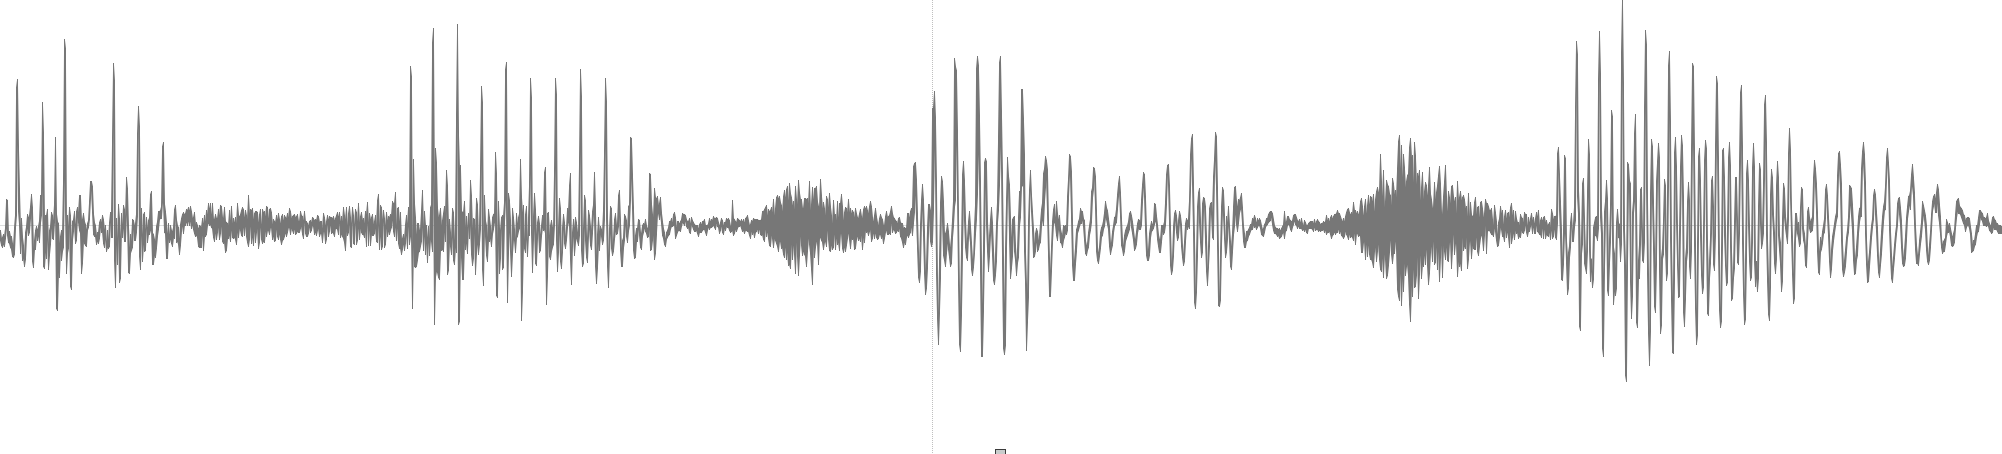
\includegraphics{chapters/sprachverarbeitung/01.png}

Ein Problem bei der Transformation von Sprache in Text ist zunächst, dass wir keine eindeutige Kodierung von der digitalen Information in das gemeinte Zeichen haben.
Dies beginnt bereits damit, dass unterschiedliche Wellenformen von Aufnahmen desselben Textes nur Ähnlichkeiten haben, aber niemals identisch sind.
Sie variieren in Lautstärke, Geschwindigkeit, Tonhöhe, Artikulation und insbesondere auch am unterschiedlichen Zeichensatz.
Denn Sprache agiert nicht mit Buchstaben, sondern mit Lauten, die von Person zu Person, z.~B.
durch regionale Dialekte bedingt, stark variieren können.
Zunächst muss einem Laut daher ein Phonem zugewiesen werden, von denen es etwa 100 gibt, und die in einem eigenen Alphabet erfasst werden können.
Hierfür gibt es mehrere, international unterschiedlich verbreitete Varianten.
Für ein Beispiel siehe z.~B. \cite[S. 1056]{russelnorvig}.

Aber selbst wenn ein Phonem identifiziert werden kann, besteht noch keine 1:1 Beziehung zwischen Phonemen und Buchstaben.
Je nach Kontext können viele Buchstaben mit verschiedenen Phonemen artikuliert werden und manche Phoneme werden durch mehrere bzw.
unterschiedliche Buchstaben repräsentiert.
Ein weiteres Problem des gesprochenen Wortes ist, dass Leerzeichen oft wegfallen.
Das heißt, Sprache bindet Wörter häufig aneinander.
Manche Buchstaben werden auch gar nicht ausgesprochen, bzw.
je nach Sprecher verschluckt.
Interpunktion wird durch Tonhöhen- und Pegelunterschiede ausgedrückt (Absenken der Stimme bei einem Punkt, Anhaben der Stimme bei einem Fragezeichen, Lautstärkeanhebung bei einem Ausrufezeichen).

\section{Methoden}
\subsection{Theoretische Grundlage: Hidden-Markov-Modelle}
Für die Erstellung eines Sprachmodells haben sich Hidden-Markov-Modelle (HMM) bewährt.
Diese sind ein einfacher Spezialfall von Bayesschen Netzen und werden verwendet, um eine probabilistische Annahme über eine zeitliche Abfolge von Zuständen zu treffen.
Ein Zustand ist eine Menge X von unbekannten Zustandsvariablen zu einem Zeitpunkt t (kurz: Xt).

Uns liegen Kenntnisse (eigentlich Annahmen, s.~u.) über frühere Zuständen zu jedem Zeitpunkt t-k (0 < k $\le$ t) vor, aus denen wir die Wahrscheinlichkeit für das Eintreten von Xt in einem Übergangsmodell erhalten.
Prinzipiell könnten wir alle Zustände von X0 bis Xt-1 (kurz: X0:t-1) auswerten.
Dies entspricht dem Übergangsmodell P( Xt | X0:t-1 ).
Da t aber unbegrenzt sein kann, wäre es notwendig, nur eine endliche Menge an vorherigen Zuständen zu betrachten.
In Bezug auf die Komplexität und den Aufwand des Modells wäre es zudem von Nutzen, die Anzahl der für die Vorhersage von Xt benötigten vorausgegangenen Zustände möglichst klein zu halten, also nur P( Xt | Xt-n:t-1 ) mit kleinem n auszuwerten.
Nach der Markov-Annahme reicht es für verschiedene Prozesse – darunter auch die Spracherkennung – völlig aus, eine Markov-Kette mit niedriger Ordnung zu verwenden.
Eine Markov-Kette n-ter Ordnung ist ein stochastischer Prozess, dessen Zustände nur von n vorherigen Zuständen abhängen.
Ein einfaches Beispiel wäre eine Markov-Kette erster Ordnung, bei der nur der unmittelbar vorausgehende Zustand für die Wahrscheinlichkeitsverteilung von Xt betrachtet wird.


Des Weiteren gehen wir davon aus, dass die Gesetze, die die Wahrscheinlichkeit für das Eintreten einer bestimmten Ausprägung von Xt auf Basis der vorherigen Zustände bestimmen, im Laufe der Beobachtung konstant bleiben, also unabhängig von t sind.
Das Modell ist also ein stationärer Prozess, für den die Übergangswahrscheinlichkeiten bereits bei der Modellierung festgelegt werden können.

Wie bereits angemerkt treffen wir nur Annahmen über die Zustandsvariablen Xt, da uns die tatsächlichen Werte xt niemals bekannt sind.
Grundlage für diese Annahmen ergeben sich nicht nur aus dem Übergangsmodell, sondern aus Beobachtungen/Messdaten, die für eine Menge von bekannten Evidenzvariablen E zu jedem Zeitpunkt t herangezogen werden.
Die Ausprägung von Et ist die Menge von Werten et.
Nach der Sensor-Markov-Annahme gehen wir davon aus, dass Et nur von Xt und nicht von weiteren Vorgängerzuständen abhängt, somit $P( Et | X0:t, E0:t-1 ) = P( Et | Xt )$ gilt.
Dies ist unser Sensormodell.
Letztlich interessiert uns aber natürlich die Gegenrichtung, also $P( Xt | Et = et )$.
Wir wollen ja Erkenntnisse über Xt gewinnen, während die Daten von Et vorliegen.

Kombinieren wir jetzt Übergangsmodell und Sensormodell ergibt sich für ein beliebiges t die Gleichung $P(X_{0:t},E_{1:t}) = P(X_0) \Sigma_{i=1}^t P(X_i | X_{i-1}) P(E_i | X_i)$.

Angemerkt sei, dass unsere Beobachtungen erst bei E1 beginnen, während wir für X0, also unseren Startzustand, eine A-priori-Wahrscheinlichkeitsverteilung P(X0) angeben.

Als Bayessches Netz lässt sich dieses kombinierte Modell z.~B. Darstellen wie in \cite[S. 665]{russelnorvig}.

Hier ist beispielsweise die Wahrscheinlichkeit, dass es an Tag t regnet 70\%, wenn es an Tag t-1 geregnet hat, und die Wahrscheinlichkeit, dass eine Person an Tag t einen Regenschirm trägt 90\%, wenn es an Tag t tatsächlich regnet.
Das Beispiel setzt voraus, dass wir nur den Regenschirm U (Evidenzvariable) beobachten können, nicht aber den Regen R (Zustandsvariable).
Ein solches Modell kann natürlich durch Erhöhung der Ordnung (Zeithorizont) und Vergrößerung der Variablenmengen (Messdaten) verbessert werden.

Diese Grundlagen des temporalen probabilistischen Schließens gelten für verschiedene Modelle, von denen uns in Bezug auf die Spracherkennung vor allem das Hidden-Markov-Modell interessiert.
In einem HMM wird der Zustand durch eine einzige diskrete Zustandsvariable abgebildet.
Das kann auch ein Wertetupel sein, in dem einzelne Variablen gebündelt werden.
Dies erlaubt die Erstellung einer Matrix für die Übergangswahrscheinlichkeiten zwischen zwei Zuständen.
Sei S die Anzahl der möglichen Zustände, so erstellen wir aus dem Übergangsmodell $P( Xt | Xt-1 )$ die $S x S$-Matrix T mit $Tij = P(Xt = j | Xt-1 = i)$, also die Wahrscheinlichkeit eines Übergangs von Zustand i in Zustand j.
Nach dem obigen Beispiel wäre das $T = P(X_t | X_{t-1}) =
\begin{pmatrix}
0,7 & 0,3 \\
0,3 & 0,7
\end{pmatrix}$.

Das Sensormodell wird als $S x S$-Diagonalmatrizen Ot dargestellt.
Zunächst benötigen wir für jeden möglichen Zustand $P( et | Xt = i )$.
Diese Werte werden in den i-ten Diagonaleintrag geschrieben:
$O_1 = \begin{pmatrix}
0,9 & 0 \\
0 & 0,2
\end{pmatrix}$;
$O_3 = \begin{pmatrix}
0,1 & 0 \\
0 & 0,8
\end{pmatrix}$.

Wobei in diesem Beispiel U1 = true und U3 = false war.

\subsection{Praktische Anwendung: akustisches Modell}
Auf der unteren akustischen Ebene müssen zunächst die Phoneme erkannt werden, d.~h.
man betrachtet den Zeitverlauf des Audiosignals und schließt anhand eines auf einem HMM beruhenden akustischen Modells auf den Inhalt.
Es wäre nicht nur zu aufwendig, sondern auch wenig hilfreich jedes einzelne Sample als Evidenzvariable zu begreifen.
Da die menschliche Sprache keine relevanten Informationen unterhalb von 100Hz liefert, bietet es sich stattdessen an, Frames dieser Länge (= 10~ms) zu bilden und die aus diesen Frames gewonnenen Informationen als Folge von Beobachtungen et zu nutzen.
Bei 44,1~kHz Samplerate enthält ein solcher Frame also 441 Samples.
Da auch die Informationen oberhalb von ca.
4 – 5~kHz für die Spracherkennung nicht mehr relevant sind, bietet auch eine geringere Samplerate von 8 – 12~kHz, wie sie in einfachen Spracherkennungssystemen oftmals verwendet wird, noch eine genügend hohe Auflösung.
Hier fasst ein Frame entsprechend 80 – 120 Samples.
Um keine relevanten Signaländerungen durch ungünstige Platzierung der Framegrenzen zu verlieren, überlappen sich die Frames.

Das Signal eines jeden Frames wird nun mittels Fourier-Transformation einer Spektralanalyse unterzogen und die Energieniveaus von 12 verschiedenen Frequenzen sowie des gesamten Frames ausgewertet.
Zusätzlich wird die Differenz zu den Werten des vorherigen Frames sowie die Differenz der Differenzen berechnet.
Folglich stehen nun 39 Werte zur Verfügung die in einem Vektor gespeichert werden und unsere Evidenzmerkmale Et für unsere Lautzustände Xt darstellen.
Somit haben wir das Sensormodell $P( Et | Xt )$ definiert.
Um aus dem Verlauf von Frames auf ein Phonem schließen zu können wird zunächst ein Übergangsmodell für Laute verwendet, das aus einem Anfang-, Mitte- und Endzustand besteht.
Damit können charakteristische Merkmale eines Lautes, wie Beginn und Endung, gut abgebildet werden.
Jeder Zustand kann durch Schleifen mehrfach hintereinander durchlaufen werden, womit sich verschieden lang gesprochene Phoneme modellieren lassen.
Jeder Laut hat sein eigenes charakteristisches Laut-HMM.
Ein Beispiel für ein Laut-HMM ist z.B. in~\cite[S. 1058]{russelnorvig} zu finden.

Wir benötigen aber nicht nur Lautmodelle, sondern auf der nächst höheren Ebene auch Übergangsmodelle für Wörter, also für jede Vokabel ein Wortmodell.
Das Prinzip ist hierbei ähnlich wie bei den Laut-HMMs, allerdings verwenden wir keine Schleifen, da Phoneme nicht ungewollt wiederholt werden.
Stattdessen benötigen wir alternative Pfade für alternative Aussprachen.
Ein Wort kann z.~B.
aufgrund einer schnellen, gebundenen Sprechweise (Koartikulation) oder aufgrund eines Dialekts unterschiedlich ausgesprochen werden.

In einem solchen Wortmodell-Graphen besteht also jeder Knoten aus einem Lautmodell.
Beide Ebenen ergeben zusammen das Übergangsmodell P( Xt | Xt-1 ).
Ein Beispiel für ein Wortmodell-Graphen ist z.~B. in~\cite[S. 1058]{russelnorvig} zu finden.

Beim Sprechen werden Worte oft aneinandergebunden (fehlende Segmentierung).
Durch ungenaue Aussprache oder sogar dem Gleichlaut zweier Worte (Homophone) besteht darüber hinaus Verwechslungsgefahr.
Es kann daher sinnvoll sein, die Wahrscheinlichkeit des Auftretens eines Wortes P(wortt) bzw.
einer Wortfolge P(wortt-n:t) im Kontext zu betrachten und die wahrscheinlichste Folge hiervon anzunehmen.
Um diese Wahrscheinlichkeitswerte zu ermitteln, bietet es sich an, auf einen Textkorpus zurückzugreifen.
Idealerweise wird dieser aus gesprochener Sprache (Transkriptionen) gespeist, da Schrifttexte oft eine andere Struktur aufweisen.
Da die Erstellung eines solchen Korpus sehr aufwendig ist und um die Komplexität der Analyse zu reduzieren, werden oft aufgabenspezifische Korpora verwendet.
Das heißt wir begnügen uns für einfachere Systeme mit denjenigen Vokabeln, die für eine gegebene Anwendung relevant sind.

\section{Sprachanalyse}
\subsection{Problemstellung}
Im vorherigen Abschnitt haben wir Grundlagen kennengelernt, wie man mittels Spracherkennung gesprochene Sprache in einen Text transformiert, wobei viele Probleme (z.~B.
Interpunktion) noch ausgeklammert wurden.
Bei der Sprachanalyse möchten wir nun einen Schritt weiter gehen und den Inhalt eines Textes logisch erfassen.
Diese Analyse erfolgt in zwei Schritten.
In einer syntaktischen Analyse ermitteln wir zunächst die Phrasenstruktur eines Satzes, um die Satzelemente in Subjekt, Prädikat und Objekt einteilen zu können.
Wir bedienen uns hierfür einer Grammatik, die eine natürliche Sprache definiert.
Mit deren Hilfe können wir einen Text parsen, das heißt ausgehend von seinen Zeichen die strukturellen Elemente identifizieren.
Wir bestimmen dabei auch weitere Satzelemente wie Attribute (Adjektive, Adverbien), Tempus, Kasus, Numerus etc.
Im nächsten Schritt wollen wir auf der semantischen Ebene mit Hilfe von Prädikatenlogik einen Zusammenhang zwischen den nun bekannten Satzelementen herstellen und damit den Inhalt des Textes schließlich erfassen.
Jedenfalls wäre dies die Idealvorstellung einer Textanalyse.
In der Praxis ergeben sich zahlreiche Schwierigkeiten.
Zunächst ist es nicht möglich ein lückenloses Vokabular und eine vollständige Grammatik einer natürlichen Sprache zu erstellen.
Natürliche Sprachen haben zahlreiche (z.~B.
regionale) Unterschiede und insbesondere das Vokabular ist in einem stetigen Fluss begriffen.
Sprecher einer Sprache halten sich selber nicht immer streng an die Sprachregeln und können meistens dennoch verstanden werden.
Grammatiken natürlicher Sprachen sind zudem hochkomplex, enthalten zahlreiche Ausnahmeregeln und sind daher nur schwer in ein festes Regelwerk zu überführen.
Wir müssen uns daher vorerst mit einer Teilmenge einer Sprache begnügen, also mit einem verkürzten Vokabular und einer reduzierten Grammatik.
Im Folgenden beschäftigen wir uns vor allem mit der englischen Sprache, da diese zu den grammatikalisch einfachsten natürlichen Sprachen gehört.
Das Textverständnis mit Mitteln der Logik ist ebenfalls schwierig zu implementieren, weil hierfür eine umfassende Logik-Datenbank der Begriffe, ihrer Bedeutungen und Zusammenhänge vorhanden sein müsste, auf die bei der Interpretation zugegriffen werden könnte.

\subsection{Methoden}
Eine Grammatik definiert eine Sprache mit Hilfe von Regeln.
Anhand dieser werden abstrakte Nichtterminalsymbole, die eine Struktur markieren, durch andere Nichtterminale und/oder Terminalsymbole (hier: die Vokabeln einer Sprache) ersetzt, bis nur noch Terminal-Symbole vorhanden sind, die einen grammatikalisch korrekten Text ergeben.
Eine solche Regel hat beispielsweise die Form $S \rightarrow a S b$.
Nichtterminale sind hier {S}, Terminale sind {a, b}.
Bei der Erstellung einer Grammatik beginnen wir bei einem Startsymbol, das sich zu feineren Strukturen und schließlich zum einem fertigen Text hin immer weiter verzweigt.
Ein Text lässt sich also in einem Ableitungsbaum darstellen, dessen Wurzel das Startsymbol bildet.
Seine inneren Knoten sind Nichtterminale und die Blätter Terminale.
Ein Ableitungsbaum für den aus obiger Grammatik erzeugten Text „aabb“ sähe entsprechend so aus:

Haben wir nun einen Text und die Grammatik einer natürlichen Sprache gegeben, können wir umgekehrt auch überprüfen, ob ein in dieser Sprache gültiger Text vorliegt, indem wir die Grammatikregeln quasi von rechts nach links betrachten.
Dabei prüfen wir, ob passende Satzstrukturen gefunden werden können.
Wir bauen den Ableitungsbaum also von den Blättern her auf.
Dieser Vorgang wird Parsen genannt, entsprechend spricht man auch von einem Parse- oder Syntaxbaum.
Auf dem Weg von den Blättern zur Wurzel des Baumes lernen wir die Satzstruktur kennen und können uns dadurch den Inhalt des Textes erschließen.
Die in vielen Implementierungen von Prolog vorhandene Erweiterung DCG (definite clause grammars) erlaubt es sehr einfach, formale Grammatiken in Prolog zu implementieren.
Die Syntax einer solchen Grammatik ähnelt dem obigen Beispiel mit kleinen Abweichungen, die sich schnell aus dem Kontext erschließen.
Im Folgenden wird die DCG-Syntax verwendet.

Betrachten wir eine sehr reduzierte Grammatik für eine Teilmenge der englischen Sprache.
Wir folgen dem Beispiel aus \cite[Kapitel 23]{bratko}.

\begin{verbatim}
sentence --> noun_phrase, verb_phrase.
verb_phrase --> verb, noun_phrase.
noun_phrase --> determiner, noun.
determiner --> [the].
noun --> [cat].
noun --> [mouse].
verb --> [hates].
\end{verbatim}

Terminale werden in DCG als Prolog-Listen in eckigen Klammern angegeben.
Prolog konvertiert diese DCG-Regeln in Prolog-Regeln.
Die erste Regel hat konvertiert die Form

\begin{verbatim}
sentence (List, Rest) :-
 noun_phrase(List, List1),
 verb­_phrase(List1, Rest).
\end{verbatim}

Abfragen für einen Text auf diese Grammatik haben die Form
\begin{verbatim}
?- sentence([the, mouse, hates, the, cat], []).
yes
\end{verbatim}

Prolog verwendet hier als Parameter Differenzlisten, also die Differenz aus List und Rest.

Fügen wir der Grammatik als zusätzliche Terminale die Pluralform der Substantive und Verben hinzu,

\begin{verbatim}
noun --> [cats].
noun --> [mice].
verb --> [hate].
\end{verbatim}

entsteht das Problem, dass unsere Grammatik noch keinen Kontext zwischen Nominalphrase und Verbphrase herstellt.
Eigentlich inkorrekte Sätze wie „the mice hates the cat“ werden noch akzeptiert (Übergenerierung).
Wir müssen den Nichtterminalen für Subjekt und Prädikat also einen Parameter für den Numerus mitgeben, der für beide Phrasen identisch ist.
In DCG lässt sich eine solche Parametrisierung folgendermaßen realisieren:

\begin{verbatim}
sentence(Number) --> noun_phrase(Number), verb_phrase(Number).
verb_phrase(Number) --> verb(Number), noun_phrase(Number1).
noun_phrase(Number) --> determiner(Number), noun(Number).
noun(singular) --> [mouse].
noun(plural) --> [mice].
verb(singular) --> [hates].
verb(plural) --> [hate].
...
\end{verbatim}


Fragen müssen ebenfalls um diesen Parameter modifiziert werden:

\begin{verbatim}
?- sentence(plural, [the, mice, hates, the, cat], []).
no
?- sentence(plural, [the, mice, hate, the, cat], []).
yes
?- sentence(Number, [the, mice, hate, the, cat], []).
Number = plural
\end{verbatim}

Je präziser eine Grammatik eine natürliche Sprache repräsentieren soll, desto aufwendiger wird auch die Konstruktion nichtterminaler Parameter.

Zur Analyse der Bedeutung eines Textes ist es wie zuvor erwähnt hilfreich, einen Syntaxbaum zu erstellen.
Ein solcher hat für das letzte Beispiel die Form

In Prolog kann ein solcher Baum mittels DCG erstellt werden, indem jedem Nichtterminal der Teilbaum als Argument übergeben wird, für den dieses Nichtterminal die Wurzel darstellt.
Unsere Grammatik wird so erweitert zu

\begin{verbatim}
sentence(Number, sentence(NP, VP)) -->
  noun_phrase(Number, NP),
  verb_phrase(Number, VP).
verb_phrase(Number, verb_phrase(Verb, NP)) -->
  verb(Number, Verb),
  noun_phrase(Number1, NP).
noun_phrase(Number, noun_phrase(Det, Noun)) -->
  determiner(Number, Det),
  noun(Number, Noun).
determiner(determiner(the)) --> [the].
noun(singular, noun(cat)) --> [mouse].
noun(plural, noun(cat)) --> [mice].
verb(singular, verb(hates)) --> [hates].
verb(plural, verb(hate)) --> [hate].
...
\end{verbatim}

Eine dazu passende Anfrage wäre

\begin{verbatim}
?- sentence(Number, ParseTree, [the, mice, hate, the, cat], []).
Number = plural
ParseTree = sentence(noun_phrase(determiner(the), noun(mice)),
            verb_phrase(verb(hate), noun_phrase(determiner(the),
            noun(cat))))
\end{verbatim}

In einem Satz stellt das Verb eine Beziehung zwischen Subjekt und eventuellen Objekten her.
Grundsätzlich unterscheidet man intransitive und transitive Verben.
Letzteren ist ein Objekt zugeordnet, auf das die Handlung des Subjekts gerichtet ist.
Die Beziehungsstrukturen einfacher Sätze lassen sich gut in Prädikatenlogik formalisieren: intransitives\_verb(subjekt), transitives\_verb(subjekt, objekt).
Der einfache Satz „Alice paints“ mit intransitivem Verb ‚paints‘ wird so zu paints(alice) umgeformt.
„Alice likes Bob“ mit transitivem Verb ‚likes‘ wird zu likes(alice, bob).
Betrachten wir nun, wie sich diese Prädikatenlogik in Prolog mit DCG darstellen lässt.
Eine Möglichkeit wäre, die Semantik aus dem Syntaxbaum herzuleiten.
Es gibt aber noch eine andere gebräuchliche Option, die Bedeutung der Syntax in der Grammatik zu enkodieren und durch nach außen sichtbare Parameter für Abfragen zugänglich zu machen.
Eine Grammatik mit der sich die einfachen Sätze „Alice paints“ und „Alice likes Bob“ und ihre Bedeutung definieren lassen, hätte mit dieser Syntax folgende Form:

\begin{verbatim}
sentence(VP) --> noun_phrase(X), verb_phrase(X, VP).
noun­_phrase(NP) --> proper_noun(NP).
verb_phrase(X, VP) --> intrans_verb(VP).
verb_phrase(X, VP) --> trans_verb(X, Y, VP), noun_phrase(Y).
intrans_verb(X, paints(X)) --> [paints].
trans_verb(X, Y, likes(X, Y)) --> [likes].
proper_noun(alice) --> [Alice].
proper_noun(bob) --> [Bob].
\end{verbatim}

Dadurch, dass wir die Bedeutung der Terminale in den Nichtterminalen als Argumente kodieren, und beim Parsen des Textes an die darüber liegenden Satzstrukturen als Parameter weiterreichen, können wir die logische Struktur eines Satzes herleiten.
Der Parameter X wird wie im Fall intrans\_verb(X, paints(X)) noch einmal separat vorangestellt, um von außen sichtbar zu sein, so dass wir eine Prolog-Anfrage auf ihn formulieren können.

Verwenden wir nicht konkret bezeichnete Subjekte (hier: bestimmte Personen), sondern abstraktere Akteure, wie ‚a woman‘ oder ‚every woman‘, so benötigen wir für den Logik-Ausdruck zusätzlich Quantoren.
„a woman paints“ müssen wir dann ausdrücken durch: Es existiert ein x, dieses x ist eine Frau und x malt $(\exists x: woman(x) \wedge paints(x))$.
Den Allquantor nutzen wir entsprechend für bspw.
„every woman likes Bob“: $\forall x: woman(x) \Rightarrow likes(x, bob)$.
Der Akteur ist hier eine Property und die Handlung eine Assertion.
Allgemein hätte eine solche Aussage in Prolog die Form exists(X, Property and Assertion) bzw.
all(X, Property => Assertion).
Für die Konstruktion einer solchen Aussage nimmt natürlich auch der grammatikalische Aufwand deutlich zu:

\begin{verbatim}
sentence(S) --> noun_phrase(X, Assn, S), verb_phrase(X, Assn).
noun­_phrase(X, Assn, s) --> determiner(X, Prop, Assn, S),
                            proper_noun(NP, Prop).
noun­_phrase(X, Assn, Assn)2 --> proper_noun(X).
verb_phrase(X, Assn) --> intrans_verb(X, Assn).
intrans_verb(X, paints(X)) --> [paints].
Determiner(X, Prop, Assn, exists(X, Prop and Assn)) --> [a].
noun(X, woman(X)) --> [woman].
proper_noun(alice) --> [Alice].
\end{verbatim}

Anfragen an diese Grammatik wären beispielsweise:
\begin{verbatim}
?- sentence(S, [a, woman, paints], []).
S = exists(X, woman(X) and paints(X))

?- sentence(S, [Alice, paints], []).
S = paints(alice)
\end{verbatim}

In diesem Beispiel wurde der Übersicht halber sogar auf Allquantoren und transitive Verben verzichtet.
Man bekommt aber bereits einen guten Eindruck davon, wie aufwendig eine solche Grammatik schon für einfache Sätze wird.
Es ist leicht einsehbar, dass eine Grammatik, die weitere grammatikalische Eigenheiten wie Tempus, Numerus, Kasus, Fragen, Befehle, Konjunktivsätze, Nebensätze (z.~B.
Beziehungen in Relativsätzen), Satzzeichen, Sonderformen und Ausnahmeregeln berücksichtigen muss, einen sehr hohen Komplexitätsgrad annimmt.
Und dabei haben wir es hier mit einer grammatikalisch noch verhältnismäßig einfachen Sprache wie Englisch zu tun.
Noch schwieriger gestaltet es sich allerdings, einen Logik-Korpus zu generieren, der die Bedeutung eines umfassenden Vokabulars einer Sprache umfasst.
Ein solches kann einschließlich Verkleinerungsformen und vergleichbaren Wortabwandlungen bis zu 1 Millionen Begriffe enthalten.
Diese müssten so kodiert sein, dass ähnliche Begriffe auch gemeinsam kategorisiert sind.
Aber auch damit wäre noch keine eigentliche Kommunikation mit einem maschinellen Agenten möglich.
Hierzu benötigt dieser zusätzlichen eine umfassende Wissensdatenbank in Logikform mit Beziehungen zwischen Begriffen, Akteuren und Weltwissen.
Offensichtlich gerät die Sprachverarbeitung hier noch an ihre Grenzen.
Daher basieren Sprachanalysesysteme, die zum Beispiel für die maschinelle Übersetzung eingesetzt werden, in der Regel auch auf probabilistischen Modellen, die große Ähnlichkeit zu den Methoden der Spracherkennung aufweisen, und zum Beispiel auf Hidden-Markov-Modellen beruhen können.

\section{Verwandte Themen}
Hidden-Markov-Modelle sind ein Spezialfall der Bayesschen Netze.
Einen weiteren Aspekt von Sprachverarbeitung ist die Digitalisierung von Schrift, sei es gedruckt oder handschriftlich.
Dies fällt aber in den Bereich der Objekterkennung/Computervision und wurde hier daher ausgeklammert.
Ähnliches gilt für die Erkennung von Gebärdensprache.

\section{Fazit}
Die Sprachverarbeitung ist gewissermaßen die Königsdisziplin in der Entwicklung künstlicher Intelligenz.
Nicht zuletzt basiert der Turing-Test auf sprachlicher Kommunikation mit maschinellen Agenten.
Dass der Turing-Test noch von keiner künstlichen Intelligenz zufriedenstellend bestanden wurde, deutet darauf hin, dass auch die Sprachverarbeitung noch vor vielen Problemen steht.
In diesem Kapitel wurden zwei Ansätze vorgestellt, die verschiedene Anwendungsfälle abdecken.
Im ersten Abschnitt wurde mit einer zustandsbasierten, probabilistischen Methode, einem Hidden-Markov-Modell, gesprochene Sprache in Text umgewandelt.
Im zweiten Abschnitt wurden Ansätze beschrieben, um Text mit Mitteln formaler Sprachen und Logik systematisch zu strukturieren und auf ihre Bedeutung hin zu dekodieren.
Während probabilistische Ansätze etwa durch Spracherkennung oder zum maschinellen Übersetzen bereits in spezifischen Einsatzbereichen gute Ergebnisse erzielen, ist die systematische Formalisierung natürlicher Sprachen und ihre Überführung in ein Logiksystem noch vor allem Forschungsgegenstand.
Es lässt sich darüber streiten, ob nicht erst mit der Entwicklung einer solchen strukturellen Sprachverarbeitung von echter künstlicher Intelligenz gesprochen werden kann, wenn also ein künstlicher Agent also nicht nur – wie im bereits bekannten Chinese Room Gedankenexperiment – lediglich Grammatikregeln befolgt, sondern seinen Wissensschatz in der Kommunikation abfragen, anpassen und erweitern kann.
Die probabilistischen Ansätze, die in der Praxis Anwendung finden, sind zwar sehr nützlich und oft recht erfolgreich, scheinen mir jedenfalls aber nur eine Simulation von Intelligenz zu darzustellen.

\section{Quellen und Literatur}
\begin{itemize}
\item Russell, Stuart / Norvig, Peter: Künstliche Intelligenz. Ein moderner Ansatz.
3., aktualisierte Auflage. München: Pearson 2012.
\begin{itemize}
\item Kapitel 15: Probabilistisches Schließen über die Zeit
\item Kapitel 22: Verarbeitung natürlicher Sprache
\item Kapitel 23: Natürliche Sprache für die Kommunikation
\end{itemize}
\item Bratko, Ivan: Prolog Programming for Artificial Intelligence.
Fourth Edition. Essex: Pearson 2012.
\begin{itemize}
\item Kapitel 23: Language Processing with Grammar Rules
(hieraus Codebeispiele im Abschnitt Sprachanalyse)
\end{itemize}
\item MIT Open Course: Artificial Intelligence. Fall 2010
\begin{itemize}
\item Lecture 14: Learning: Sparse Spaces, Phonology
\url{http://ocw.mit.edu/courses/electrical-engineering-and-computer-science/6-034-artificial-intelligence-fall-2010/lecture-videos/lecture-14-learning-sparse-spaces-phonology/}
\end{itemize}
\end{itemize}
